\documentclass[12pt]{article}
\usepackage[letterpaper,top=2cm,bottom=2cm,left=3cm,right=3cm,marginparwidth=1.75cm]{geometry}
\usepackage{graphicx} % Required for inserting images
\usepackage[french]{babel} 
\usepackage[T1]{fontenc}
\usepackage{float} % Pour forcer les images à être là où il faut.
\usepackage{listings} % Listes
\usepackage{color} % Couleurs
\usepackage{xcolor} % Couleurs
\usepackage{lipsum}
\usepackage{amsmath} % Math
\usepackage{amssymb} % Math
\usepackage{amsmath}  % Math
\usepackage{multicol} % Pour les colonnes
\usepackage[hidelinks]{hyperref} % Hyperlien
\usepackage[
backend=biber,
style=alphabetic,
sorting=ynt
]{biblatex}
\addbibresource{biblio.bib} % Bibliographie

% Commandes Math
\newcommand{\K}{\mathbb{K}}
\newcommand{\N}{\mathbb{N}}
\newcommand{\C}{\mathbb{C}}
\newcommand{\R}{\mathbb{R}}
\newcommand{\Rd}{\mathbb{R}^d}
\newcommand{\I}{\mathbf{I}}
\newcommand{\dcrochetg}{[\![}
\newcommand{\dcrochetd}{]\!]}
\newcommand\independent{\protect\mathpalette{\protect\independenT}{\perp}}
\def\independenT#1#2{\mathrel{\rlap{$#1#2$}\mkern2mu{#1#2}}}
\newtheorem{thm1}{Théorème}[section]
\newtheorem{lemme1}[thm1]{Lemme}
\newtheorem{prop1}[thm1]{Proposition}
\newtheorem{rmq1}{Remarque}
\newtheorem{exemple1}{Exemple}
\newtheorem{defin1}{Définition}
% Fin commandes Math

\begin{document}


\begin{titlepage}
    \centering
    {\huge\bfseries Projet Météorites\par}
    \vspace{1cm}
    {\scshape\Large Rapport de projet tutoré\par}
    \vspace{1.5cm}
    {\large Yanis Petit, Rassem Djimadoum, Duc-Khoi Nguyen \& Garance Malnoë\par
    encadrés par Jean-François Coeurjolly\par}
    \vspace{0.5cm}
    {\large Master 1 SSD\par}
    \vspace{0.5cm}
    {\large Janvier - Avril 2025\par}
    \vspace{3cm}
\end{titlepage}
\pagenumbering{gobble}
\tableofcontents
\clearpage
\pagenumbering{arabic}
\section{Introduction}
Ce rapport présente le projet tutoré réalisé de Janvier à Avril 2025 dans le cadre de notre première année de Master SSD, encadré par Jean-François Coeurjolly.  Notre projet porte sur l'étude du jeu de données "Meteorite Landigs" provenant de la Meteoritical Society (Société Météoroligique) qui est disponible sur l'\href{https://data.nasa.gov/Space-Science/Meteorite-Landings/gh4g-9sfh/about_data}{\underline{Open Data de la NASA}}.\\
\\
Nous n'avions pas d'objectif défini pour ce projet, l'idée première était d'explorer le jeu de données et de choisir le(s) sujet(s) nous intéressant(s)  mais plusieurs idées nous avaient été suggrées lors du premier rendez-vous avec Jean-François Coeurjolly :\\
\begin{itemize}
	\item[-] Faire étude temporelle des données : détecter la présence d'une saisonnalité ou d'une tendance par exemple.\\
	\item[-] Etudier les liens entre différentes variables par exemple l'impact de la masse.\\
	\item[-]Créer un modèle permettant de prédire le nombre de métoérites tombées dans un pays à partir de sa superficie, ses coordonnées de latitude et 		longitude.\\
	\item[-] Réaliser une étude spatiale pour déterminer si certaines régions sont plus touchées et le cas échéant essayer de déterminer la source des différences.\\
\end{itemize}
Nous commençons par présenter notre organisation, les outils, les langages ainsi que le détail des bibliothèques que nous avons utilisés pour le projet. Nous présentons ensuite les résultats de l'exploration des données (analyses unvariées et multivariées). Nous nous interessons ensuite à la modélisation en 3D du jeu de données. Ensuite, nous regardons la modélisation de Rassem. Enfin, nous concluons ce rappport par une étude de l'impact environnemental du projet. \\
\\

\section{Organisation, Outils, bibliothèques R et Python}
Organisation : rendez-vous avec Jean-François, répartition du travail, cours de gestion de projet (mermaid chart, plannification).\\
\\
Outils : GitHub, Python, R, VSCode, RStudio. Expliquer que l'on a travaillé en R et en Python parce qu'on est à 4 sur le projet, qu'on maitrise tous les quatre les 2 langages et que l'on a profité des avantages et libraires proposées par les 2 langages.Python pour l'exploration du jeu de données et la modélisation de Rassem parce que package déjà proposés. R pour la visualisation end 3D car package et possibilité de faire une application Shiny.\\
\\
Packages Python : lister.\\
\\
Packages R : lister.\\ 
\\

\section{Exploration des données}
Le jeu de données est composé de 45716 entrées décrites par neuf variables :
\begin{itemize}
\item[-] \textbf{name} (qualitative nominale): le nom de la météorite.
\item[-] \textbf{nametype} (qualitative binaire) : "Valid" ou "Relict", Relict signifie qu'il s'agit d'un objet très déformé qui est probablement d'origine météorite.
\item[-] \textbf{recclass} (qualitative nominale) : le type de la météorite.
\item[-] \textbf{mass} (quantitative continue) : la masse de la météorite en grammes.
\item[-] \textbf{fall} (qualitative binaire) : indique si on a observé la chute de la météorite (fell) ou si elle a été trouvée au sol (found).
\item[-] \textbf{year} (quantitative continue) : l'année où la météorite a été rescencée.
\item[-] \textbf{reclat} (quantitative continue) : latitude où la météorite a été trouvée.
\item[-] \textbf{reclong} (quantitative continue) : longitude où la météorite a été trouvée.
\item[-]\textbf{geoLocation} : couple de la latitude et de la longitude.\\
\end{itemize}
La première étape de notre projet a été d'explorer les données afin de mieux les comprendre et d'essayer de trouver des liens entre eles variables dans le but de choisir un angle d'approche à donner à notre projet. Nous avons donc commencé par une analyse univariée de chaque variable en regroupant les variables reclat, reclong et geoLocation.\\
\\
Pour cette partie, nous avons utilisé Python avec les packages numpy, pandas, geopandas, plotly et shapely pour faire les analyses univariées et multivariées. Le code se trouve sur le fichier exploration.ipynb disponible sur le Git.\\
\\
\subsection{Analyses univariées}
\subsubsection{Name}
Il n'y a pas de données manquantes pour le nom des météorites et elles ont toutes un nom unique. Par curiosité, nous avons regardé la répartition du choix de la première lettre :
\begin{figure}[H]
\centering
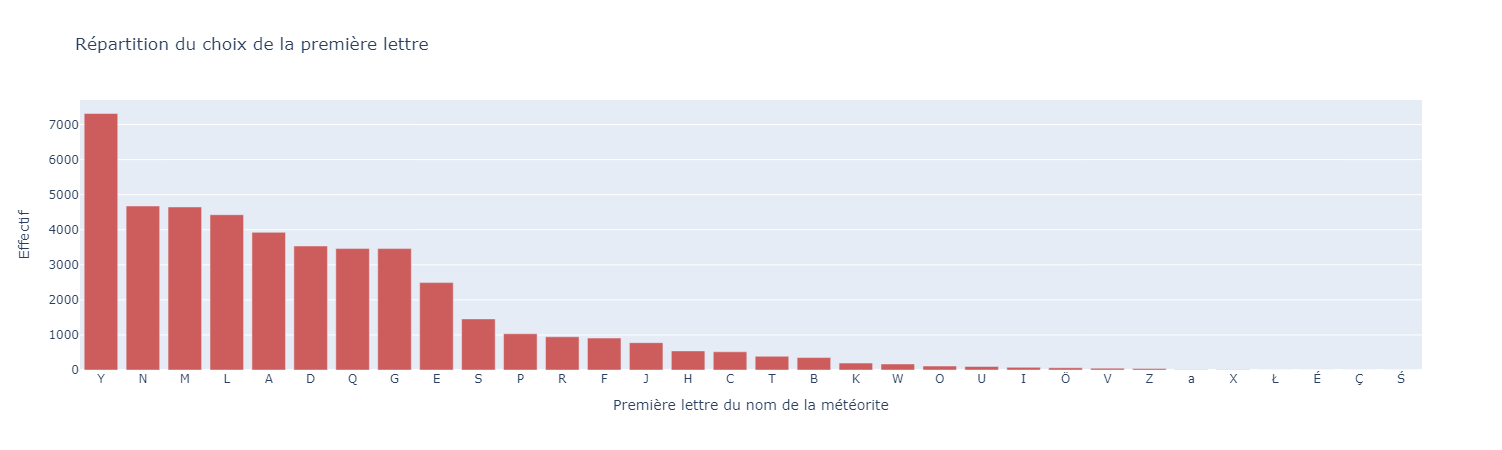
\includegraphics[width=15cm]{Images/exploration/name_barplot_lettres.png}
\caption{Diagramme en barres du choix de la première lettre du nom des météorites}
\end{figure}
\subsubsection{Nametype}
Cette variable n'a pas de données manquantes. Comme expliqué précédemment, c'est une variable qualitative binaire décrivant si la météorite a bien été identifiée comme valide (Valid) ou s'il s'agit d'un objet fortement déformé qui est probablement d'origine météorite (Relict). Une large majorité de entrées du jeu de données sont considéréees comme valides : 45641 météorites valides soit 99,8\% contre 75 "Relict" soit 0,02\%.
\subsubsection{Recclass}
Il n'y a pas de données manquantes pour la variable recclass qui correspond au classement de la météorites. Le jeu de données compte 422 classes différentes mais certaines sont largement majoritaires :
\begin{figure}[H]
\centering
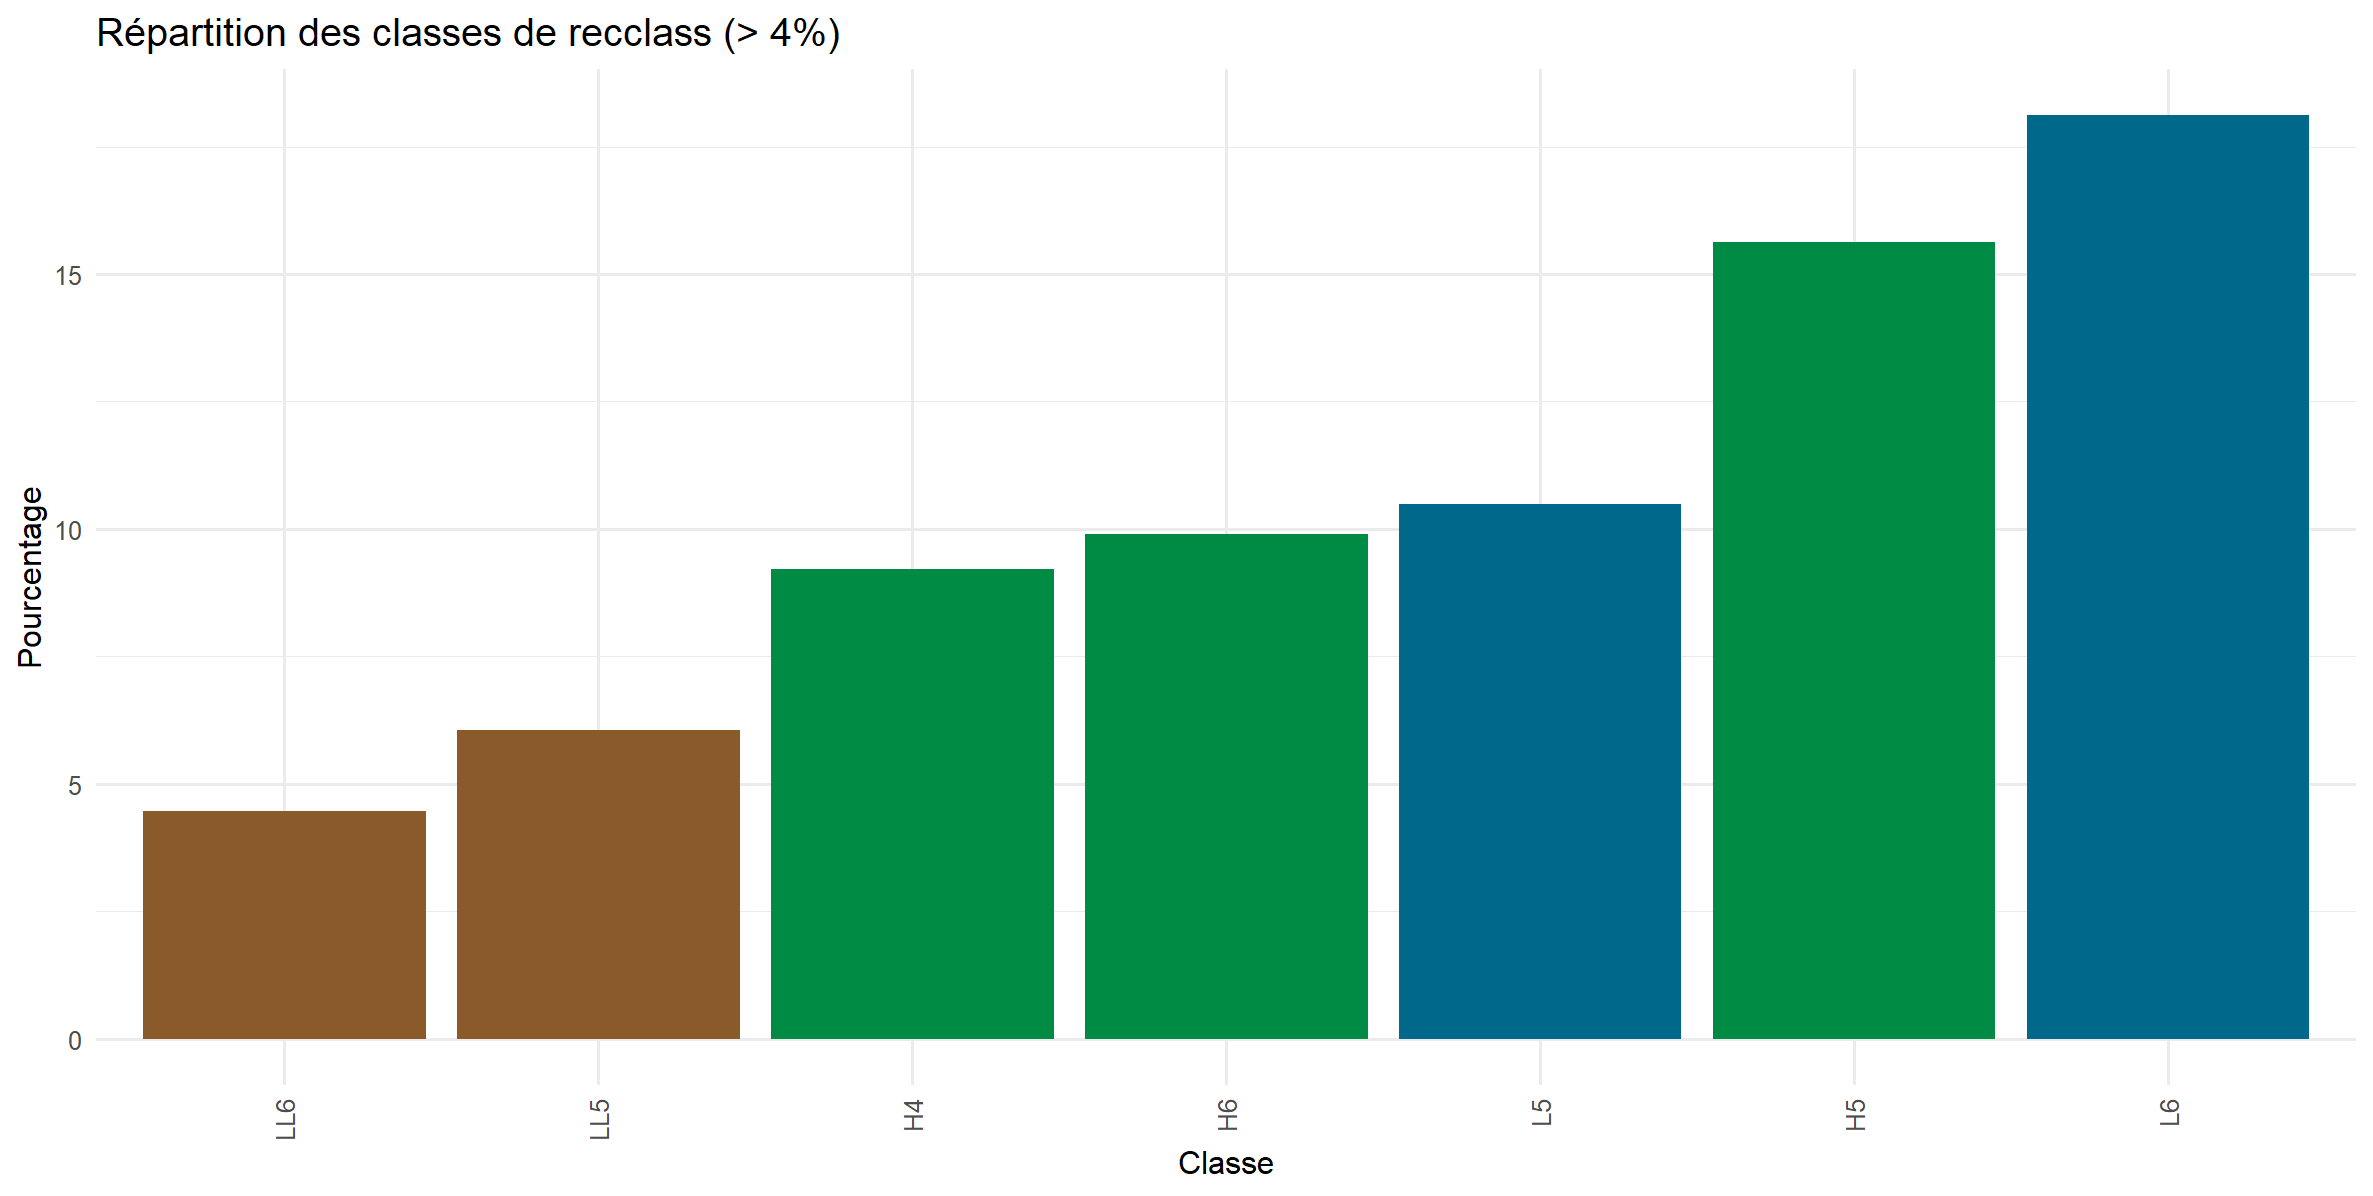
\includegraphics[width=15cm]{Images/exploration/recclass_piechart_class.png}
\caption{Piechart des classes de météorites}
\end{figure}
Chercher signification des classes les plus populaires.
\subsubsection{Mass}
Nombre de données manquantes : 131.
\subsubsection{Fall}
Pas de données manquantes
\subsubsection{Year}
Nombre de données manquantes : 291.
\subsubsection{Location}
Nombre de données manquantes : 7315 (il manque à la fois lat, long et geolocation). On va regrouper ici l'analyse de la position dans l'espace et de la latitude et de la longitude.

\subsection{Analyses multivariées}
Reprendre les graphiques et les textes fait sur exploration.ipynb + ajouter un équvalent de pairs en Python ?

\subsection{Discussion des limites du jeu de données}

L'étude des données manquantes nous a montré qu'il manquait essentiellement des données sur la masse, l'année et la localisation de la chûte. Même en supprimant toutes les lignes avec au moins une valeur manquante, nous avons toujours 38115 éléments (83\%), ce qui est a priori suffisament grand pour pouvoir faire des analyses pertinentes.\\
\\
On se rend compte que les météorites sont sans doutes pas du tout toutes répertoriées. Problème : le site de la NASA (et ailleurs sur internet) on a pas d'information sur la formation du jeu de données, on ne sait pas si ce sont des données rapportées par tout un chacun ou si ce sont seulement les données rapportées par des téléscopes / scientifiques.\\
\\
On voit bien avec la carte par point que l'on a très peu de données dans les régions où il y a personne : déserts, forêt amazonienne, chine rurale. L'antarctique est une exception, cela est lié au fait qu'il y ait des recherches sur les météorites là bas. Citation, explications liées au projet lien vers le papier / l'article. On peut supposer que les grosses météorites sont + probables d'être vues/repérées que les météorites faisant seulement quelques grammes (lien vers le papier sur la dégradation des météorites dans l'atmosphère ?) une fois sur le sol.\\
\\
Pas possible de faire une étude temporelle car 1. on a seulement l'année ou est tombée la météorite (lié au fait qu'elles soient essentiellement trouvées une fois tombées ?) 2. on observe une forte augmentation du nombre de météorites répertoriées à partir des années 1970 alors que le jeu de données commence en 1640. On a alors cherché un autre jeu de données plus complet pour la partie temporelle. Nous avons trouvé le jeu de données MetCat (lien). Explication du jeu de données metcat, variables disponibles. Mais plusieurs problèmes sont resortis lors de l'analyse de ce jeu de données : 1. la temporalité n'est pas très précise (mois =  Printemps ou Juin-Août) 2. Si on se restreint aux données correctement labelisées on en a finalement très peu et très étalées dans le temps (précision, il faut finir l'analyse du jeu de données.


\section{Visualisation en 3 dimensions}
Travail de Yanis et Duc-Khoi.

Capture d'écran des possibilités de visualisation que nous proposons + lien vers une page hébergeant l'application shiny ?

\section{Modélisation de processus ponctuels}
Travail de Rassem

\section{Conclusion}
\section{Remerciements}
\section{Références}
\printbibliography
- Lien vers l'article sur les météorites en Antartique.
\section{Impact environnemental et sociétal du projet}
J'ai remis les consignes du pdf de l'Ensimag. Cette section doit représenter envrion 20\% du rapport.
\subsection{Impact environnemental personnel}
Partie moins importante.
Estimation de l'impact des trajets domicile-travail, impact de la consommation des équipements utiliés (ordinateurs perso/fixes, temps d'utilisation des serveurs github,...), autres impacts.
Expression en exprimé en kg eq. CO2.

\subsection{Impact global du projet}
Dans cette section, nous vous demandons d’évaluer l’impact global du projet sur lequel vous avez travaillé. Si vous avez travaillé sur un produit fini (logiciel, infrastructure…), vous devrez mettre en valeur non seulement l’impact du produit lui-même mais également l’évolution de cet impact entre le début et la fin de votre PFE. Si vous avez travaillé sur une preuve de concept, un avant-projet, un projet de recherche et développement ou un projet de recherche pure, votre évaluation devra tenir compte des possibles utilisations de votre travail dans un contexte applicatif. Cette section sera la plus importante de la partie consacrée à l’impact environnemental et sociétal. Nous ne vous demandons pas une simple évaluation technique, mais une véritable réflexion déclinée sur deux plans :
1. à petite échelle (concernant uniquement votre projet, à court terme)
2. à plus grande échelle (long terme, et dans l’hypothèse où le même type de projet venait à se généraliser et/ou
se transposer dans différents secteurs)
Nous demandons dans cette section un avis honnête, critique et argumenté sur les impacts positifs et négatifs du projet. Vous ne serez pas évalué sur la quantité ni la qualité des bonnes pratiques sociales et environnementales mises en œuvre dans le cadre de votre PFE : il est donc inutile d’écoblanchir votre discours. Ce qui nous importe est la vision critique que vous adoptez.

\subsection{Politique de la structure d'acceuil}
Dans cette section, nous vous demandons de dresser une liste des actions menées par la structure d’accueil sur les aspects écologiques et sociaux. Cela peut concerner des actions individuelles ou la mise en œuvre d’une véritable politique dans ce domaine. De même, cela concerne à la fois des politiques extérieures éventuelles (fondations, dons à des organismes…), mais également des actions destinées à l’ensemble des collaborateurs de l’entreprise (conditions de travail, mise en œuvre de bonnes pratiques environnementales au quotidien…). Vous mettrez bien entendu en évidence tous les aspects positifs de cette politique. En revanche, si vous estimez qu’il y a des voies d’amélioration possibles en termes de politique de responsabilité sociale et environnementale, nous vous encourageons à proposer une liste d’actions concrètes qui pourraient être mises en œuvre. Cela montrera non seulement votre capacité à réaliser une analyse critique, mais cela vous permettra également d’être une force de proposition pour votre structure d’accueil.
\newpage
\section{Annexe}
\end{document}